\documentclass{article}
\renewcommand{\thesection}{\Roman{section}} 

% if you need to pass options to natbib, use, e.g.:
% \PassOptionsToPackage{numbers, compress}{natbib}
% before loading nips_2017
%
% to avoid loading the natbib package, add option nonatbib:
% \usepackage[nonatbib]{nips_2017}

%\usepackage{main}

% to compile a camera-ready version, add the [final] option, e.g.:
\PassOptionsToPackage{square,numbers}{natbib}
\usepackage[final]{main}

\usepackage[utf8]{inputenc} % allow utf-8 input
\usepackage[T1]{fontenc}    % use 8-bit T1 fonts
\usepackage{hyperref}       % hyperlinks
\usepackage{url}            % simple URL typesetting
\usepackage{booktabs}       % professional-quality tables
\usepackage{amsfonts}       % blackboard math symbols
\usepackage{nicefrac}       % compact symbols for 1/2, etc.
\usepackage{microtype}      % microtypography
\usepackage{multicol}
\usepackage{graphicx}
\usepackage{amsmath}
\usepackage{bbm}
\usepackage{enumerate}
\usepackage{adjustbox}
\usepackage{enumitem}
%\usepackage[margin=0.5in]{geometry}
%\DeclareMathOperator*{\argmax}{argmax}
\usepackage{listings}
\usepackage{color}
\usepackage{listings}% http://ctan.org/pkg/listings
\lstset{
  basicstyle=\ttfamily,
  mathescape
}
 
\definecolor{codegreen}{rgb}{0,0.6,0}
\definecolor{codegray}{rgb}{0.5,0.5,0.5}
\definecolor{codepurple}{rgb}{0.58,0,0.82}
\definecolor{backcolour}{rgb}{0.95,0.95,0.92}
 
\lstdefinestyle{mystyle}{
    backgroundcolor=\color{backcolour},   
    commentstyle=\color{codegreen},
    keywordstyle=\color{magenta},
    numberstyle=\ttfamily\tiny\color{codegray},
    stringstyle=\color{codepurple},
    basicstyle=\ttfamily\small,
    columns=fullflexible,
    breakatwhitespace=false,         
    breaklines=true,                 
    captionpos=t,                    
    keepspaces=true,                 
    numbers=left,                    
    numbersep=5pt,                  
    showspaces=false,                
    showstringspaces=false,
    showtabs=false,                  
    tabsize=4,
}
 
\lstset{style=mystyle}
\graphicspath{{images/}}
\title{Big Data Science - Spring 2018\\
       \Large Assignment 1}
%\graphicspath{{images/}}
\setcitestyle{round, sort, numbers}

% The \author macro works with any number of authors. There are two
% commands used to separate the names and addresses of multiple
% authors: \And and \AND.
%
% Using \And between authors leaves it to LaTeX to determine where to
% break the lines. Using \AND forces a line break at that point. So,
% if LaTeX puts 3 of 4 authors names on the first line, and the last
% on the second line, try using \AND instead of \And before the third
% author name.

\author{
  Daniel Rivera Ruiz\\
  Department of Computer Science\\
  New York University\\
  \href{mailto:drr342@nyu.edu}{\texttt{drr342@nyu.edu}}\\
}

\begin{document}

\maketitle

% \cite{} - in-line citation author, year in parenthesis.
% \citep{} - all citation info in parenthesis.

%	\begin{figure}[ht]
%		\centering
%		\frame{
%            \includegraphics[width=1.0\linewidth]{tree.png}
%       }
%		\caption{Classification results for the sentence \textit{"There are slow and repetitive parts, but it has just enough spice to keep it                  interesting."} using the Stanford Sentiment Treebank. As can be seen, sentiment scores are available for each phrase.}
%		\label{tree}
%	\end{figure}

\section{Basic Knowledge and High-level Architectural Questions}
    \begin{enumerate}[label=(\alph*)]
        \item Forty+ Concepts: Enrich your Analytics Glossary.\\
        Research, briefly explain and define the following concepts in your own words:
        \begin{enumerate}[label=\textbf{\arabic*.}]
        
            \item \textbf{\textit{Prescriptive Analytics}}\\
Prescriptive analytics is the third phase of the business analytics process, succeeding the descriptive and predictive phases.\\
While descriptive analytics focuses only on historical data and predictive analytics uses this data in order to anticipate future events, prescriptive analytics cares not only about what will happen, but also about why will it happen. Making use of data and mathematical models, along with business knowledge, prescriptive analytics can help take advantage of a future opportunity or mitigate a future risk.\\
The nature of prescriptive analytics is a dynamic one, meaning that new data, better algorithms, and other changing factors are constantly taken into account in order to improve the predictions of the models and suggest better options for the decision-making process. 

            \item \textbf{\textit{Kafka}}\\
Kafka is a distributed stream processing platform developed by Apache that allows its users to publish and subscribe to streams of records in real-time and in a fault-tolerant way. It is mainly used to build real-time streaming data pipelines and the applications that interact with them.

            \item \textbf{\textit{Apache Spark}}\\
Spark is an open source processing engine designed to be powerful, fast and easy to use. It was developed at UC Berkley in 2009 and its main application is big data analytics. It provides APIs for some of the most commonly used technologies such as Java, Python and Scala, on top of which several modules are built in order to provide specific functionalities such as SQL DataFrames, streaming, machine learning and graph computation.

            \item \textbf{\textit{Neural Networks}}\\
A neural network is an information processing paradigm inspired by the way nervous systems (such as the brain) process information. The key element of this paradigm is its structure to process information, which is composed of a large number of highly interconnected processing elements (neurons) working in unison to solve specific problems.\\
Neural networks, like people, learn by example, which means that they must be configured for a specific application, such as pattern recognition or data classification, through a learning process. This process, just as in biological systems, involves adjustments to the synaptic connections that exist between the neurons. In artificial neural networks, these adjustments require the training of weights, which define how much influence a given input has on the output of the neuron.\\
Figure \ref{nn} depicts a fully-connected neural network with three units in the input layer, four units in the hidden layer, and two units in the output layer.
	\begin{figure}[ht]
		\centering
		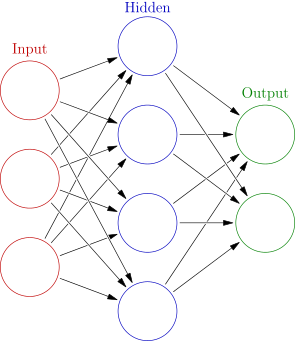
\includegraphics[width=0.5\linewidth]{nn.png}
		\caption{Neural Network Model.}
		\label{nn}
	\end{figure}
	
            \item \textbf{\textit{Big Data}}\\
Big data is a concept that refers to sets of data so big that the traditional computational techniques for data processing are not sufficient to analyze them and find valuable patterns in them. For a data set to be considered big data, it must be characterized by the three so called \emph{V dimensions}: volume, variety and velocity. Lately, two more dimensions have started to be considered as well: veracity and value.\\
The main reason behind the emerging of big data science was the need to manipulate huge amounts of data (both structured and unstructured) in order to create statistical reports and predictive models that are used for decission-making in a wide range of businesses and industries.

            \item \textbf{\textit{Trust Based Recommender Systems}}\\
Trust-based recommender systems are collaborative systems based on user relations who express trust between them. The Epinions website, for example, recommends items to a user that were previously liked by trusted users. The trust between two users means that one user believes on the utility of the recommendation of another.
            
            \item \textbf{\textit{Linear Regression}}\\
Linear regression is an statistical model used to approximate the relation of dependency between a bounded variable $Y$, the unbounded variables $X_i$ and an aleatory term $\epsilon$. The model can be expressed as follows:
    \begin{equation*}
        Y_t = \beta_0 + \beta_1 X_1 + \beta_2 X_2 + \ldots + \beta_p X_p + \epsilon
    \end{equation*}
Where $Y_t$ is the bounded or regressed variable, $X_1, X_2, \ldots, X_p$ are the unbounded variables or regressors, and $\beta_0, \beta_1, \ldots, \beta_p$ are the parameters of the regression, which measure the influence of each unbounded variable on the bounded variable.\\
In the classical approach to the model, the parameters $\beta_i$ are selected such that the sum of the squares of the errors (the difference between an observation $Y$ and the prediction of the model $\hat{Y}$) is minimized.\\
Figure \ref{linear} shows a basic example of a linear regression with only one independent variable.
	\begin{figure}[ht]
		\centering
		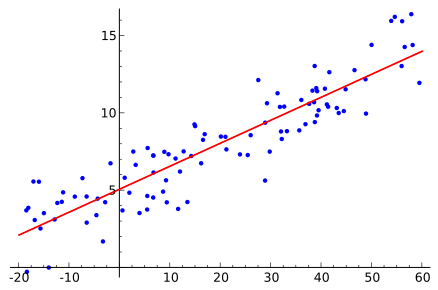
\includegraphics[width=0.5\linewidth]{linear.png}
		\caption{Linear Regression Model.}
		\label{linear}
	\end{figure}
	
            \item \textbf{\textit{Gradient boosting}}\\
Gradient boosting is a machine learning technique used for linear regression analysis and statistical classification problems. The idea behind it is to generate a predictive model in the form of a set of weaker models, typically decision trees. The model is built in a staggered manner as it is usual in boosting methods, and it allows for the optimization of an arbitrary differentiable loss function.\\
To understand how gradient boosting works, the easiest example is the least squares problem in linear regression, where the objective is to minimize the mean squared error $(\hat{y}-y)^2$. At each step of gradient boosting, there is an imperfect Model $F_m$ that the algorithm will improve on by adding an estimator $h$ to provide a better model: $F_{m+1}(x) = F_m(x) + h(x)$.\\
The ideal selection for $h$ would be such that $h(x) = y - F_m(x)$, making the new model correctly predict the expected value and therefore correcting its predecessor. These residuals of the form $y-F(x)$ are in fact the negative gradients with respect to $F(x)$ of the squared error loss function $\frac{1}{2}(y-F(x))^2$ and can be generalized to other loss functions in what is known as \emph{gradient descent algorithm}. 
            
            \item \textbf{\textit{Knowledge Discovery}}\\
Knowledge discovery refers to the process of  searching large volumes of data for patterns that can be considered valuable knowledge. It was developed as part of the data mining domain and is closely related to it both in terms of methodology and terminology. It is also known as knowledge discovery in databases (KDD), and it creates abstractions of the input data, which may in turn become additional data that can be used for further usage and discovery.
            
            \item \textbf{\textit{Class Label (in Data Classification)}}\\
The term class label is usually used in the context of supervised machine learning, in particular in classification problems, where a set of examples of the form \textit{(attribute values, class label)} is given, and the goal is to learn a rule that predicts the label given a set of attribute values. In contrast to linear regression, where the predicted (bounded) variable can take on an infinite number of values, the class label is always restricted to a finite (discrete) set of values.
            
            \item \textbf{\textit{KNN (K nearest neighbor)}}\\
The method of the k-nearest neighbors (knn) is a supervised classification algorithm that is used to estimate the probability density function of a given element $x$ belonging to a class $C$. There are no suppositions about the distribution of the elements, and the learning process is considered to be "lazy", meaning that the function is approximated only locally and the computation process is reserved for the classification stage.\\
The training examples for the algorithm are vectors in a multidimensional space, where each dimension is associated to an attribute of the examples. A point in this space is assigned to class $C$ if it is the most frequent class among the $k$ nearest training examples. To measure the vicinity, euclidean distance is commonly used.\\
The best selection for the value $k$ depends mainly on the data: larger values of $k$ reduce the effect of noise in the classification but also introduce less resolution to distinguish among similar classes.\\
Figure \ref{knn} shows a simple example of the k-nearest neighbors algorithm. For $k = 3$, the circle would be assigned to the triangle category, whereas with $k=5$ it would be assigned to the square category.
	\begin{figure}[ht]
		\centering
		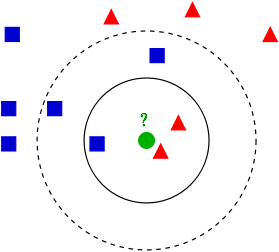
\includegraphics[width=0.5\linewidth]{knn.png}
		\caption{K-Nearest Neighbors Algorithm.}
		\label{knn}
	\end{figure}
	
            \item \textbf{\textit{Analytic}}\\
Analytic, in the context of computer science, refers to an application of statistics dedicated to solve decision-making problems within the context of an information system. Originally it was strongly related to computer systems, but in recent years it has evolved into the field of data mining. Mathematics are essential for the algorithms used in analytics, which basically try to extract useful information out of huge amounts of data.

            \item \textbf{\textit{Hadoop 2.0}}\\
Hadoop is a project developed by Apache intended as an open-source software for reliable, scalable, distributed computing. The Hadoop software library is a framework that allows for the distributed processing of large data sets across clusters of computers using simple programming models. Rather than rely on hardware to deliver high-availability, the library itself is designed to detect and handle failures at the application layer, which delivers a highly-available service on top of a cluster of computers, each of which may be prone to failures.
            
            \item \textbf{\textit{Deep Belief Networks}}\\
In the fields of machine learning and artificial intelligence, a deep belief network (DBN) is a kind of generative graphic model within the family of deep neural networks. It is characterized by having several hidden layers which are interconnected among themselves, but with no connections between units of a single layer. DBNs can be used in unsupervised classification problems, since they are capable of detecting features in the inputs and reconstruct them probabilistically. Furthermore, after the learning process has been completed, the DBN can be trained again in a supervised manner in order to enhance the classification process.
            
            \item \textbf{\textit{Deep Learning}}\\
Deep learning refers to a set of algorithms within the machine learning domain that tries to model high-level data abstractions using complex architectures based on multiple non-linear transformations.\\
Deep learning is a part of a wider set of machine learning techniques based on understanding data representations. The main objective of deep learning is to identify which representations of a given piece of data are better (facilitate the analysis and learning processes) and how to develop models to recognize these representations.\\
Several deep learning architectures such as deep (convolutional) neural networks have been applied to challenging tasks like computer vision and speech recognition, yielding state of the art results in most of them.
            
            \item \textbf{\textit{Convolutional Neural Networks}}\\
A convolutional neural network (CNN) is a kind of artificial neural network where the neurons correspond to receptive fields in a similar fashion to real neurons in the visual cortex of a biological brain. This kind of network is a variation of a multi-layer perceptron with bi-dimensional matrices , which have prooven to be very effective for tasks like artificial vision and image classification and segmentation.\\
CNNs consist of several layers of convolutional filters of one or more dimensions. After each layer, it is common to add a function to perform a non-linear mapping. When used as classification networks, it is usual to find two phases: one for feature extraction and sampling reduction, and one for the final classification over the extracted features, which consists mainly of regular perceptron neurons. As the data goes through the convolutional and feature reduction layers, their dimensionality is reduced, making the neurons in farther layers less sensitive to noise in the input data, but at the same time more complex in the sense of the features that activate them.

            \item \textbf{\textit{Feature Selection}}\\
In machine learning, feature selection refers to the process of selecting a subset of relevant features (predicting variables) to be used in the building of models. Feature selection techniques are used mainly to simplify the models and make them easier to interpret, to reduce training time, and to improve generalization performance by reducing overfitting.\\
Feature selection techniques arise from the premise that the data contains several redundant or irrelevant features that can be removed without incurring in information loss. They are not to be confused with feature extraction techniques, which are used to generate new features as function of the original ones.
            
            \item \textbf{\textit{Business Intelligence}}\\
Business intelligence (BI) comprises all the strategies, applications, products, technologies and technical architectures that are focused on managing and creating knowledge about the environment through analyzing the data available in a business or organization.\\
One of the key ideas behind BI is the difference between data, information and knowledge, with data being the vaguest concept (e.g. 10,000), information something more precise (e.g. The sales in April were \$10,000), and knowledge being extracted out of information by analyzing it (e.g. April was the month with the lowest sales of the year).\\
Once knowledge has been obtained through analyzing the information coming from all the areas of an organization, it is possible to establish strategies and determine strengths and weaknesses.

            \item \textbf{\textit{Cross-validation}}\\
Cross-validation is a technique used to evaluate the results of an statistical analysis and guarantee that they are independent of the partition between training and test sets. It consists of repeating and calculating the arithmetic mean obtained from the evaluation measures over different partitions, and it is used in environments where the main objective is maximizing the precision of the model to predict unseen examples. It is a widely used technique to validate projects in artificial intelligence and machine learning.\\
Cross validation originated as an improvement over the holdout method, which consists on dividing the data into two complementary subsets, using one of them for training and the other for testing. This method, however, is not very efficient since it depends heavily on the data available and the way the partition is made.\\
K-fold cross validation, one of the most common types of cross validation, improves over holdout by dividing the sample in $K$ subsets. One of the subsets is used as the test set and the rest as the training set. This procedure is repeated over $K$ iterations, using each of the subsets as the test set one at a time. Finally, the arithmetic mean of all the iterations is reported as the result of the method. Figure \ref{cross} shows an example of how K-fold cross validation is performed for $k=4$.
	\begin{figure}[ht]
		\centering
		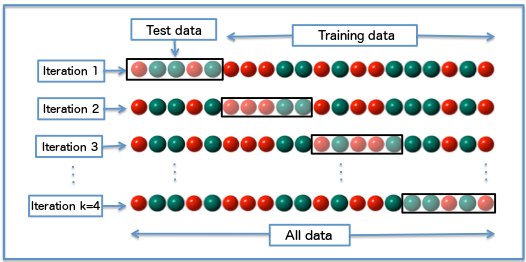
\includegraphics[width=0.5\linewidth]{cross.jpg}
		\caption{K-fold Cross Validation.}
		\label{cross}
	\end{figure}
            
            \item \textbf{\textit{Graph Database}}\\
A graph database is a kind of database that represents all its information as nodes in a graph and the relationships between the data as the edges. With this representation, graph theory can be used to traverse the database, which describes attributes of both the nodes (entities) and the edges (relationships).\\
Some of the advantages of a graph database are the following: they allow for wider queries, which are not limited to tables. There is no need to define a specific number of attributes. Registers can have variable length, avoiding the need to define a size without wasting space. The database can be traversed hierarchically, obtaining for instance the grandparent node of a node and vice versa. 
            
            \item \textbf{\textit{Confusion Matrix}}\\
In the fields of artificial intelligence and machine learning, a confusion matrix is a tool that allows the visualization of the performance of an algorithm that is used for supervised learning tasks. Each column of the matrix represents the number of predictions of each class, while each of its rows represents the instances of the real class. One of the benefits of confusion matrices is that they allow to easily identify if the system is confusing two classes.\\
If the amount of samples in the input data differ greatly from one class to another, the error rate of the classifier may not be representative of how good it is performing. If, for instance, there are 990 sample of class 1 and only 10 samples of class 2, a classifier predicting always 1 will get a 99\% precision. This doesn't mean, however, that the classifier is doing a good job, since it has a 100\% error rate at classifing samples of class 2. 
            
            \item \textbf{\textit{Split Validation}}\\
In the context of machine learning, split validation refers to the process of randomly assigning data points to two complementing sets $S_0$ and $S_1$, usually called training set and test set. The size of each of the sets is arbitrary although typically the test set is smaller than the training set. The objective of split validation is to use $S_0$ to train the algorithm, and afterwards use $S_1$ to test the performance of the algorithm on a previously unseen test set.  
            
            \item \textbf{\textit{Sentiment Analysis}}\\
Sentiment analysis, also known as opinion mining, refers to the use of natural language processing (NLP), text analysis and computational linguistics in order to identify and extract subjective information from text resources. From the text mining perspective, sentiment analysis is a task of massive automated classification of documents, in function of the positive or negative connotation of the language used throughout the document. It is important to mention that sentiment analysis usually relies on statistical and association relationships, rather than linguistic analysis.\\
In general terms, sentiment analysis tries to determine the attitude of a speaker or writer towards a certain topic, or the general contextual polarity of a given document. This attitude can be a judgment or opinion, an emotional mood, or an emotional communicative intention.
            
            \item \textbf{\textit{Feature (in data analytics)}}\\
In the fields of data analytics and machine learning, a feature is an individual property of an observed phenomenon that can be measured. The selection of discriminant features, with high informative value and independent from each other, is a crucial step towards obtaining an efficient algorithm for tasks such as pattern recognition, classification and regression.\\

            \item \textbf{\textit{Semi-Structured Data}}\\
Semi-structured data is a form of data that does not comply with the formal structure of models associated to relational databases or other forms of data tables. They are characterized for having tags or markers that separate semantic fields and impose hierarchies among the registers and fields of the data.\\
The most common examples of semi-structured data are XML or JSON documents, that are widely used throughout the internet to transmit data entities that belong to the same class but may have different attributes whose order is not important.
            
            \item \textbf{\textit{Structured Data}}\\
Structured data refers to any data that resides in a fixed field within a record or a file. This includes data contained in relational databases and spreadsheets. A data model is associated to structured data that specifies which data will be recorded and how it will be stored, processed and accessed, making it easy to enter, query and analyze.\\
Examples of structured data are any fields that can be found in a relational database: name, date, address, numbers, currency, etc.
            
            \item \textbf{\textit{Unstructured Data}}\\
Unstructured data are basically all the other data that do not fit in the previous categories, meaning that they can take any form and size without having to adhere to a rigid structure or predefined format. Examples of unstructured data include photos and images, videos, webpages, text, audio, etc.
            
            \item \textbf{\textit{Data Clustering}}\\
Data clustering refers to the task of grouping a set of objects in such a way that members of the same group (denominated \emph{cluster}) are similar to each other in some way. It is one of the main tasks within the filed of exploratory data mining and is commonly used in several fields like statistical analysis, machine learning, pattern recognition, information retrieval and bioinformatics, among others.\\
Data clustering does not refer to a specific algorithm, but rather to the task of grouping itself, which can be accomplished using several algorithms that differ significantly in the idea of what is a group and how to identify them efficiently. Classical ideas of a group include small distances among members of the group, dense areas of the data space, and specific statistical distributions.
            
            \item \textbf{\textit{Granger Causality}}\\
Granger causality is a statistical concept of causality that is based on prediction. According to Granger causality, if a signal $X_1$ "Granger-causes" a signal $X_2$, then past values of $X_1$ should contain information that helps predict $X_2$ above and beyond the information contained in past values of $X_2$ alone. Its mathematical formulation is based on linear regression modeling of stochastic processes.\\
In figure \ref{granger} we can observe a series $X$ that "Granger-causes" series $Y$, since the patterns observed in the former are approximately repeated in the latter after some time lag. Therefore, future values of $Y$ can be predicted by using past values of $X$.
	\begin{figure}[ht]
		\centering
		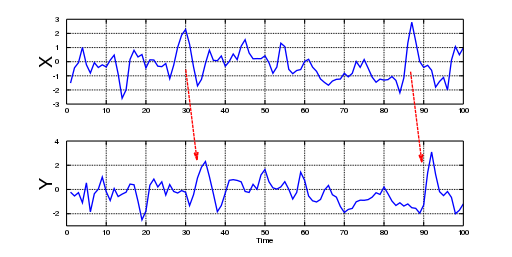
\includegraphics[width=0.75\linewidth]{granger.png}
		\caption{Granger Causality Example.}
		\label{granger}
	\end{figure}
            
            \item \textbf{\textit{Data Classification}}\\
In machine learning and statistics, classification refers to the problem of selecting from within a set of categories (labels) the one that best fits a new observation, based on a set of data that contains observations whose labels are known. Typical examples of classification problems include determining whether an e-mail is or not spam, or giving a diagnosis to a patient given their observed characteristics and symptoms.\\
Usually, the individual observations are analyzed within a set of quantifiable features that can be categorical or numerical. An algorithm that implements classification is known as a classifier, which can be thought of as a mathematical function that maps the input data to a category.
            
            \item \textbf{\textit{Supervised Learning}}\\
In machine learning and data mining, supervised learning refers to a technique used to identify a function that can predict an output value corresponding to any given valid input. The function is first presented with a set of training data that will use during its learning process, after which it will be able to generalize to previously unseen situations.\\
The two most common examples of supervised learning problems are linear regression and classification. In the first case, the output of the function is a numerical value, where as in the second the output is a label identifying a class or category.
            
            \item \textbf{\textit{Triplestore}}\\
A triplestore or RDF store is a type of database that is specifically designed to store and retrieve triples by means of semantic queries. A triple is a data entity consisting of a subject, a predicate and an object, like "John is 28" or "John knows Mary". Just like in a relational database, information can be retrieved using a query language, but in this case the storage is optimized to retrieve triples.
            
            \item \textbf{\textit{Unsupervised Learning}}\\
Unsupervised learning is a technique used in machine learning where a model is designed to fit a set of "unlabeled" input observations. It differs from supervised learning by the fact that there is no a priori knowledge of the output expected and therefore the accuracy of the model is not usually measured.\\
The most common applications of unsupervised learning are density estimation in statistics, and clustering and dimensionality reduction in machine learning. It can also be used together with supervised learning techniques in complex problems where only partially observed data is available.
            
            \item \textbf{\textit{Training Data vs Test Data (in the context of cross validation)}}\\
Training data refers to the set of examples or observations that are used to fit the parameters of a machine learning model. The model uses these examples in an iterative manner to compare its predictions with the target values and modify its parameters accordingly.\\
The test data set, which must always be independent of the training data set but follow the same probability distribution, is used to evaluate the performance of the algorithm. If a model fits the test data set well it usually means that the training process was successful. A test set is therefore only used to assess the performance of the algorithm, i.e., to know how well it generalizes to previously unseen data.
            
            \item \textbf{\textit{Deep Learning}}\\
Deep learning refers to a set of algorithms within the machine learning domain that tries to model high-level data abstractions using complex architectures based on multiple non-linear transformations.\\
Deep learning is a part of a wider set of machine learning techniques based on understanding data representations. The main objective of deep learning is to identify which representations of a given piece of data are better (facilitate the analysis and learning processes) and how to develop models to recognize these representations.\\
Several deep learning architectures such as deep (convolutional) neural networks have been applied to challenging tasks like computer vision and speech recognition, yielding state of the art results in most of them.
            
            \item \textbf{\textit{Ensemble Methods}}\\
In statistics and machine learning, ensemble methods are a technique that uses multiple learning algorithms to yield a better performance in its predictions compared to what any one of the constituent algorithms could obtain by themselves. A machine learning ensemble allows for a flexible structure to exist among the set of alternative models that comprise it, which makes it relatively easy to implement.
            
            \item \textbf{\textit{ETL Jobs}}\\
Extract, Transform and Load (ETL) is the process that allows organizations to move data from multiple sources, format them and clean them, and load them into another database, data mart or data warehouse to be analyzed or to be used as part of a business process. ETL processes can also be used in the integration of legacy systems. A recent development in ETL is the implementation of parallel processing, which has improved the overall performance of this processes, specially when large volumes of data are being handled.
            
            \item \textbf{\textit{SQL}}\\
Structured Query Language (SQL) is a domain specific language that grants access to a management system of relational databases and allows to perform operations on them. One of its main characteristics is the ability to handle algebra and relational calculus, which in turn allows to perform queries to retrieve and modify information within the databases.\\
SQL consists of a data definition language, a data manipulation language and a data control language. Its scope includes data insertion, queries, updates and deletion, as well as creation and modification of schemes and data access control.
            
            \item \textbf{\textit{Alternative Data (in the financial investment context)}}\\
Alternative data refers to data used by hedge fund managers and other institutional investment professionals to obtain insight into an investment process.These data sets contain information about a particular company that is published by external sources, which can provide unique and timely insights into investment opportunities.\\
Alternative data sets are often categorized as big data because of their size and complexity, and because they are usually compiled from various sources such as financial transactions, sensors, mobile devices, satellites, public records and the internet.
            
            \item \textbf{\textit{CRISP-DM}}\\
Cross Industry Standard Process for Data Mining (CRISP-DM) refers to a process model that describes the approaches used by data mining experts and that has become the de facto standard for data mining development and knowledge discovery projects.\\
CRISP-DM divides the data mining process in six main phases: business understanding, data understanding, data preparation, modeling, evaluation and deployment. However, the data mining process continues even after the deployment phase, since the lessons learned throughout the process can lead to new business questions, which will in turn generate valuable insight that will benefit both current and future data mining processes. 
        \end{enumerate}
    \end{enumerate}
    
\section{Questions from the readings and use cases}
    \begin{enumerate}[label=(\alph*)]
        \item Hash Joins.
        \begin{enumerate}[label=\arabic*.]
            \item Explain in your own words the concept of Hash Joins. Provide an example. Describe the differences between Hash Joins and Normal SQL Join.\\
\newline
A hash join is performed by acquiring one data set and converting it into the equivalent of an in-memory single-table hash cluster (assuming there is enough memory) using an internal hashing function on the join column(s) to generate the hash key. Then the data from the second table is acquired, applying the same hashing function to the join column(s) while reading each row, and checking to see whether it exists a matching row in the in-memory hash cluster. Since a hashing function is being used on the join column(s) to randomize the distribution of data in the hash cluster, a hash join can only work when the join condition is an equality. The first table is referred to as the build table (it is used to “build” the in-memory hash cluster), and the second table is known as the probe table (it is used to “probe” the in-memory hash cluster).\\
A hash join is almost invariably described as a join mechanism that does tablescans, but this is not a necessity, since the data sets can also be acquired through an indexed access path. Another of the comments that is made too casually is that a hash join is good for joining a small table to a large table: the comment about small and large tables should really be stated in terms of the small and large data sets that are extracted from the tables.\\
The following snippet of pseudo-code shows a simple example of how hash join works in two tables $R$ and $Q$:
        \begin{lstlisting}
/* Hash relation $R$ */
for each tuple $r \in R$ do
    put $r$ in bucket no. $h(r.A)$
endfor

/* Probe relation $Q$ */
for each tuple $q \in Q$ do
    for each tuple r in bucket no. $h(q.A)$ do
        if $r.A = q.B$ then
            put $r \circ q$ in the output relation
        endif
    endfor
endfor \end{lstlisting}

The main difference between a hash join and a normal SQL join, which is commonly referred as a nested loop join, is that in the latter there are two nested loop constructs. The outer loop works through table 1 and the inner loop works (possibly many times) through table 2. Because of the structure of this algorithm, the two tables in a nested loop are commonly referred to as the outer table and the inner table . The outer table is also commonly referred to as the driving table.
\newline

            \item Explain this statement: \emph{the computational cost of a Hash Join depends on the cost of building the hash table.}\\
\newline
As it can be observed in the pseudo-code example in the previous question, there are two parts to a hash join algorithm: building the hash table and probing it. If we take a look at the probing part, we identify that it looks a lot like a nested loop join, with the main difference that the inner for loop does not traverse all the elements in the first table, but rather only the ones in the current "bucket". What this meas is that the efficiency of the hash join algorithm depends largely on how the hash table is built. For instance, if the hash table has a poor design with too few or too many buckets, then the whole algorithm will degrade to a nested loop join.\\
If we expect the probe part of the hash join to be efficient, we have to build a good hash table, and therefore the statement \emph{the computational cost of a Hash Join depends on the cost of building the hash table.} This means that if the hash table is properly built and if both tables have similar sizes, the overall complexity of the whole algorithm will be similar to the complexity of building the hash table alone.
        \end{enumerate}
    \end{enumerate}
    
\section{Real Case Scenario for Data Analytics Life-cycle Project}
    \begin{enumerate}[label=(\alph*)]
        \item Uplifting Models and the 2012 Obama’s Campaign.
        \begin{enumerate}[label=\arabic*.]
            \item Describe \emph{uplifting models} in details and in your own words, their advantages and disadvantages. Explain how uplifting models were used in the 2012 political campaign.\\
\newline
Uplifting models originate from the assumption that effective campaigns should be directed selectively to those who, with high probability, will respond positively (e.g., buy a product or visit a web site). Properly targeted campaigns will give a greater return on investment than a randomly targeted one, and what is even more important, they will not annoy those who are not interested in the offer. 

According to uplifting models, a customer database can be divided into four groups:
\begin{itemize}
    \item Persuadables: customers that responded because of the action.
    \item Sure things: customers that would have responded regardless of the action (unnecessary costs).
    \item Lost causes: customers that did not respond and the action had no impact (unnecessary costs).
    \item Do not disturbs: customers that did not respond because the action had a negative impact (e.g. a customer got annoyed by the campaign, might even have churned).
\end{itemize}

Traditional models such as propensity models or response models are not capable of distinguishing these four groups, while uplift models can. This is because traditional models predict the conditional class probability $P(\textit{response}|\textit{treatment})$, while uplift models predict the change in behavior resulting from the action $P(\textit{response}|\textit{treatment}) - P(\textit{response}|\textit{no treatment})$.

To build an uplifting model, a random sample (the treatment dataset) of customers is selected and subjected to the marketing action. A disjoint sample is also selected (the control dataset), to which the action is not applied, and which serves as the background against which the results of the action will be measured. The model is now built for predicting the difference between class probabilities on the two sets of data.

Uplift models have proven to be effective, but there are certain considerations that make them more difficult to implement than traditional models: 
\begin{itemize}
    \item It generally is more complex to find a group of Persuadables than Sure Things.
    \item In the case of voters, many undecided voters may fall into the group of Persuadables and can be switched to your candidate and motivated to vote when given a particular treatment.
    \item It's more difficult to measure the success of the model because it's attempting to measure the influence that the treatment caused to change a customer's behavior.
    \item The measurement of the model's success might be biased since the treatment and control datasets could be conformed by completely different customers. 
\end{itemize}

One of the most famous cases where uplifting models have been used was President Obama's 2012 presidential campaign. The campaign's data analyst used uplifting models to heavily target voters who were most likely to be influenced by contact. Afterwards, they used personalized messages via several channels of contact such as social media, television, direct mail, and telephone. This campaign was a clear example of how efforts can be concentrated to influence the group of Persuadables. In the end, the heavy investment made in this kind of campaign paid off with quite positive results.\\

            \item Explain how uplifting models can be applied in Marketing.\\
\newline
Marketing is the most straightforward application for uplifting models. As it was briefly explained in the previous answer, a targeted marketing campaign will result in bigger profits than a regular one, since the costs of the campaign itself will be significantly reduced by addressing only the customers that are more likely to have a positive response to the campaign.\\
In other words, uplifting models can help the marketing team of an organization to classify its customers into the four categories described above. Once the classification is completed, the marketing campaign needs only be directed to the persuadable customers, since these are the only ones who will in fact be positively influenced by it, which will translate in increased revenue while minimizing the marketing costs.\\
Furthermore, the classification process is one that needs constant tuning and improvement. Therefore, once a targeted campaign has been implemented, its results can be analyzed and used to further improve the classification algorithm, which will in turn result in better outcomes for future campaigns.\\
Another important application and one of the most effective uses of uplifting models is in the removal of negative effects from retention campaigns. Both in the telecommunications and financial services industries, retention campaigns can often trigger customers to cancel a contract or policy. Uplifting models allows these customers (do not disturbs) to be removed from the campaign.
\newline
        \end{enumerate}
        \item Data Understanding in Behavioral Analytics.\\
        Consider the situation where you will help a business identify their customers’ cluster type: (1) Loyal Customers, (2) Discount Customers, (3) Lost Causes, (4) Sure Things, (5) Sleeping Dogs and (6) Persuadables.
        \begin{enumerate}[label=\arabic*.]
            \item Define each type of these customers (explain how each customer of the above type has a unique behavior).\\
\newline
\begin{itemize}
    \item \textit{\textbf{Loyal Customers.}}\\
    This type of customers is less in numbers but promote more sales and profit as compared to other types, since they are the ones which are completely satisfied and keep coming back for more. It is crucial to interact and keep in touch with them on a regular basis to leverage their experience and learn what makes them so satisfied with the business. They will recommend the business or product to friends and family, sending a healthy stream of new customers to the organization.
    \item \textit{\textbf{Discount Customers.}}\\
    Discount customers are also frequent visitors but they are only a part of business when offered with discounts on regular products and brands or they buy only low cost products. The more the discount, the more they tend towards buying. These customers are mostly related to small industries or industries that focus on low or marginal investments on products. In order to retain this type of customers, it is important to provide added value that will make them think twice before switching to another company.
    \item \textit{\textbf{Lost Causes.}}\\
    Lost causes are the customers that have ceased the business relationship with the organization. This loss of customers, commonly referred as customer churn, can be either voluntary or involuntary. Voluntary churn occurs when the customer decides to switch to another company, while involuntary churn occurs due to external circumstances such as a customer's relocation. When it comes to addressing customer churn situations, companies usually concentrate on voluntary churn, because it typically occurs due to factors of the company-customer relationship that can be controlled, such as how billing interactions are handled or how after-sales help is provided.
    \item \textit{\textbf{Sure Things.}}\\
    Sure customers are the ones that will continue to buy the products or services of the organization, regardless of the actions taken to retain them. Because of this condition, uplifting models try to identify sure thing customers in order to remove them from the targeted marketing campaign. Unlike loyal customers, sure thing customers will not necessarily recommend the organization, but rather limit themselves to continue the ongoing  business relationship.
    \item \textit{\textbf{Sleeping Dogs.}}\\
    Also known as do not disturb customers, sleeping dogs are customers that are better left alone. Contacting this type of customers may cause a negative response like provoking them to cancel a subscription, return a product, or ask for a price adjustment. In the context of uplifting models, it is very important to identify the sleeping dogs and remove them from the targeted campaign, not only because they will not respond favorably to it, but because of the counterproductive reaction that may arise. 
    \item \textit{\textbf{Persuadable Customers.}}\\
    Persuadable customers are the ones who can be convinced to purchase, but will only do so if they are contacted at the right moment. They are the main target of a campaign designed using uplifting models, since the revenue that they generate is contingent upon the success of the campaign. In a sense, a persuadable customer is the opposite of an sleeping dog: while the sleeping dogs will continue to purchase only if they are not contacted, the persuadable customers must be contacted in order to encourage them to buy.
    \newline
\end{itemize}

            \item Explain in details the data sources (unstructured vs. structured) you will need to be able to apply data clustering to identify these customer’s types.\\
\newline
I believe that the most important data sources to identify these type of customers would be information of the customers' credit card transactions, along with sales records from the company.\\
To identify, for instance, customers in the sure things and loyal categories, we could simply check the databases for credit card transactions that occur on a regular basis. The discount customers can also be easily identified by cross-referencing regular purchases of discounted products, and it would even be possible to identify which products the customers are usually buying, in order to offer them similar deals in the future. The case of the lost causes requires a little bit more of analysis, since we first need to identify which customers used to do business with the company and no longer do, and additionally check their credit card history to see if they are now buying the same products elsewhere.\\
Identifying sleeping dogs and persuadable customers can probably be the most challenging task. In the case of sleeping dogs, we should be looking for customers that are only subscribed to a regular service that is renewed automatically, or perhaps customers that only purchase online. For the persuadables it would be important to identify transactions that are far apart from one another (in contrast to sure things and loyals which are regular) and especially if they are related to some sort of promotion or if they are complemented by similar purchases at other companies (which would mean that the customers are still not sure which company they prefer).\\
Since identifying these two categories can be the most challenging, additional information can then be introduced to find similarities among customers and try to predict more sleeping dogs or more persuadables making use of the cases that have already been identified. Looking at demographic information of the customers (age, gender, neighborhood where they live, etc.) along with their purchase history (average purchase total, favorite products, time of day and day of the week when they purchase, etc.) a similarity measurement could be devised in order to be able to make predictions of the kind \emph{if customer A has been identified as a sleeping dog, and customer B is similar to customer A, then customer B is likely to be a sleeping dog as well}.\\
This kind of analysis could also be implemented to predict the other customer categories, but since it requires a lot more effort, it would probably only be worth implementing for the most crucial classes.
\newline

            \item Bonus (+15pts). Provide a sample data sets and a design process (following CRISP-DM) on how you will be using the dataset to cluster customers and later predict a new unknown customers type.\\
\newline
Assuming that the data sets containing all the relevant information about customers and transactions are available, a design process using the CRISP-DM standard could look as follows:
\begin{itemize}
    \item \textbf{\textit{Business understanding.}}\\
    In the first stage of the process the main objective is to define the hypothesis we will try to prove based on our knowledge of the business. In this case we will try to prove that there is another category, aside from the six already described, to which customers of the company can be assigned.
    \item \textbf{\textit{Data understanding.}}\\
    Once we have formulated the hypothesis, it is important to get familiar with the data that is available to us, in order to identify which portions will be useful for the analysis stage. Understanding the data means knowing exactly what can and can't be done with it, knowing how much of it is available and in what format, but must importantly, knowing why do we need it and what do we need it for.
    \item \textbf{\textit{Data preparation.}}\\
    This is the most time-consuming stage of the process and is the foundation of the modeling stage: if the data that we feed to the model is not adequate, the model is likely to perform poorly. Therefore, in this stage we will pre-process the data to make sure it is exactly what we need. For instance we need to make sure that numerical data is properly formatted and not stored as a string, we need to identify if there are missing values in the databases and decide what are we going to to with them. We also need to select the features that are more relevant to our model and select the parts of the data that are more useful accordingly.
    \item \textbf{\textit{Modeling.}}\\
    Once the data is ready we can proceed to the modeling stage of the process. For the task at hand the most straightforward approach is to develop a $k$-means clustering model with $k = 7$. Once the model is trained and the clusters have been defined, we should be able to identify (by looking at the labels of the data) which cluster corresponds to which category. The remaining cluster will have to be the one that the model is proposing as the new customer category.
    \item \textbf{\textit{Evaluation.}}\\
    In order to evaluate the model and determine if there is in fact another category of customers, a holistic analysis of the results would have to be performed. At this point, the business understanding of the problem becomes very useful again, since it will provide the guidelines to decide if the new category proposed really has characteristics that make it unique and that can be valuable for the company.
    \item \textbf{\textit{Deployment.}}\\
    Finally, if the updated model with the seventh category is found to provide a significant improvement over the previous one, it can be defined as the new standard to classify existing and new customers. However, regardless of the results of the process, it is important to remember that the CRISP-DM is an iterative process, which means that the whole cycle would have to be repeated again several times. It could be, for instance, that after analyzing the previous results, some modifications can be made to the modeling or the data pre-processing stages in order to further improve the implementation of the solution.
\end{itemize}

        \end{enumerate}
    \end{enumerate}

\nocite{*}
\bibliography{main} % path to your bib file (without .bib extension!)
\bibliographystyle{plainnat} % bib style (IEEE, APA, etc.)

\end{document}